\documentclass[10pt,a4paper]{article}

\usepackage[utf8]{inputenc}
\usepackage[T1]{fontenc}
\usepackage{amsmath}
\usepackage{amsfonts}
\usepackage{amssymb}
\usepackage{graphicx}
\usepackage{hyperref}
\usepackage{listings}
\usepackage{xcolor}
\usepackage{float}
\usepackage[top=2cm, bottom=2cm, left=2cm, right=2cm]{geometry}

\title{Knowledge Graphs Project: Research Publication Domain}
\author{Jonàs Salat, Albert Vidal}

\begin{document}

\maketitle

\section{Exploring DBpedia}
[This section is for exploration purposes only, no deliverables required]

\section{Ontology Creation}
\subsection{TBOX Definition}
The TBOX (Terminological Box) defines the schema, classes, and properties of our knowledge graph. It serves as the structural foundation for our ontology.

\begin{figure}[H]
    \centering
    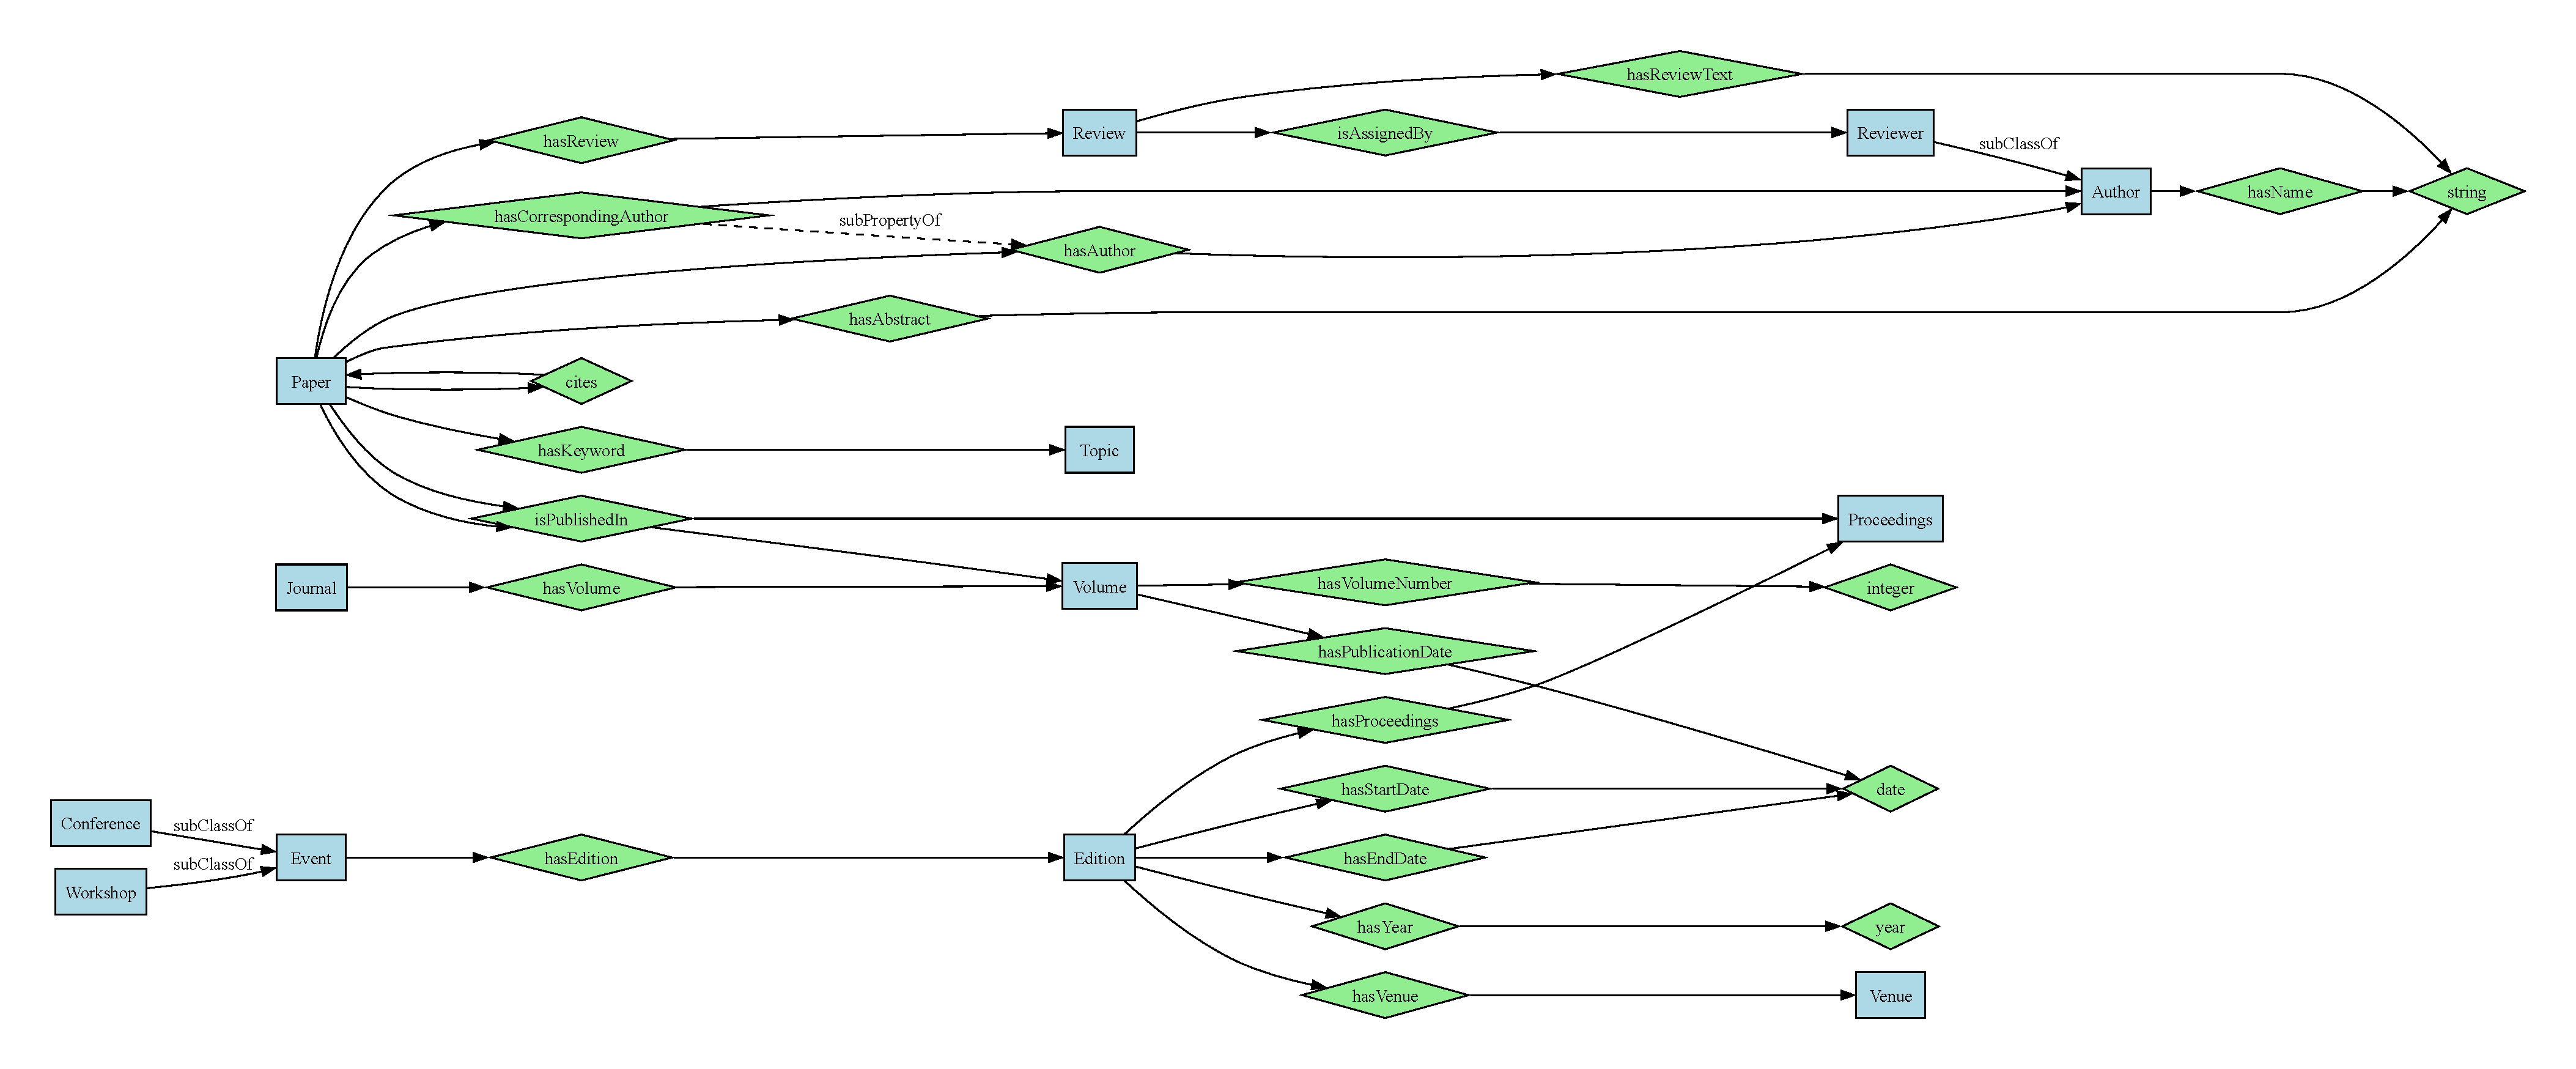
\includegraphics[width=\textwidth]{img/publication_tbox.pdf}
    \caption{Visualization of the Publication Domain TBOX showing classes, properties, and their relationships. Classes are shown in light blue boxes, properties in light green diamonds, and subclass/subproperty relationships with dashed lines.}
    \label{fig:tbox}
\end{figure}

\subsubsection{Classes}
The TBOX defines the following main classes:
\begin{itemize}
    \item \textbf{Paper}: A research paper
    \item \textbf{Author}: A person who writes papers
    \item \textbf{Event}: An academic event where research is presented
    \item \textbf{Conference}: A well-established research forum (subclass of Event)
    \item \textbf{Workshop}: A forum for exploring new trends (subclass of Event)
    \item \textbf{Edition}: A specific instance of a conference or workshop
    \item \textbf{Journal}: A periodical publication
    \item \textbf{Volume}: A collection of papers in a journal
    \item \textbf{Proceedings}: A collection of papers from a conference/workshop edition
    \item \textbf{Review}: An evaluation of a paper
    \item \textbf{Reviewer}: A scientist who reviews papers (subclass of Author)
    \item \textbf{Topic}: A subject area of a paper
    \item \textbf{Venue}: A location where an edition takes place
\end{itemize}

\subsubsection{Properties}
The TBOX defines various properties to establish relationships between classes:

\paragraph{Paper Properties}
\begin{itemize}
    \item \textbf{hasAbstract}: Links a paper to its abstract (domain: Paper, range: string)
    \item \textbf{hasKeyword}: Links a paper to its topics (domain: Paper, range: Topic)
    \item \textbf{cites}: Links a paper to papers it cites (domain: Paper, range: Paper)
    \item \textbf{isPublishedIn}: Links a paper to its publication venue (domain: Paper, range: Proceedings or Volume)
    \item \textbf{hasAuthor}: Links a paper to its authors (domain: Paper, range: Author)
    \item \textbf{hasCorrespondingAuthor}: Links a paper to its corresponding author (domain: Paper, range: Author, subproperty of hasAuthor)
    \item \textbf{hasReview}: Links a paper to its reviews (domain: Paper, range: Review)
\end{itemize}

\paragraph{Author Properties}
\begin{itemize}
    \item \textbf{hasName}: Links an author to their name (domain: Author, range: string)
\end{itemize}

\paragraph{Event Properties}
\begin{itemize}
    \item \textbf{hasEdition}: Links a conference/workshop to its editions (domain: Conference/Workshop, range: Edition)
\end{itemize}

\paragraph{Edition Properties}
\begin{itemize}
    \item \textbf{hasVenue}: Links an edition to its venue (domain: Edition, range: Venue)
    \item \textbf{hasStartDate}: Links an edition to its start date (domain: Edition, range: date)
    \item \textbf{hasEndDate}: Links an edition to its end date (domain: Edition, range: date)
    \item \textbf{hasYear}: Links an edition to its year (domain: Edition, range: year)
    \item \textbf{hasProceedings}: Links an edition to its proceedings (domain: Edition, range: Proceedings)
\end{itemize}

\paragraph{Journal Properties}
\begin{itemize}
    \item \textbf{hasVolume}: Links a journal to its volumes (domain: Journal, range: Volume)
\end{itemize}

\paragraph{Volume Properties}
\begin{itemize}
    \item \textbf{hasPublicationDate}: Links a volume to its publication date (domain: Volume, range: date)
    \item \textbf{hasVolumeNumber}: Links a volume to its number (domain: Volume, range: integer)
\end{itemize}

\paragraph{Review Properties}
\begin{itemize}
    \item \textbf{isAssignedBy}: Links a review to its assigner (domain: Review, range: Reviewer)
    \item \textbf{hasReviewText}: Links a review to its text content (domain: Review, range: string)
\end{itemize}

\subsubsection{Inverse Properties}
The following inverse relationships are defined:
\begin{itemize}
    \item \textbf{isPublishedIn} and \textbf{containsPaper}
    \item \textbf{hasEdition} and \textbf{isEditionOf}
    \item \textbf{hasVolume} and \textbf{isVolumeOf}
\end{itemize}

\subsection{ABOX Creation}
\label{sec:abox}

The ABOX (Assertional Box) of our knowledge graph was created by processing and transforming the provided CSV datasets into RDF triples. The implementation handles the complex relationships between different entities while ensuring data integrity and consistency.

\subsection{Implementation Details}

The ABOX creation process begins by loading all CSV files into pandas DataFrames for efficient data manipulation. Each entity type is processed sequentially, with careful attention to maintaining referential integrity between related entities. The implementation uses a custom URI generation function that creates deterministic, unique identifiers for each entity by hashing their primary keys.

For topics, we extract unique keywords from the papers dataset and create corresponding Topic instances. This approach ensures that each keyword appears only once in the knowledge graph, regardless of how many papers use it. Venues are similarly deduplicated, with each unique venue name creating a single Venue instance.

The author creation process handles both required and optional attributes. While author ID and name are mandatory, email addresses are added only when available. This pattern of handling optional attributes is consistently applied throughout the implementation, ensuring that the knowledge graph only contains valid, non-null data.

Conference and Workshop instances are created as separate entities, each with their own unique identifiers. The implementation maintains a clear distinction between these event types while ensuring they can be properly linked to their respective editions and papers.

Edition instances are created with careful validation of their relationships to venues and events. The implementation ensures that each edition is properly associated with a valid venue and includes temporal information (year) when available. This temporal aspect is particularly important for maintaining the chronological integrity of the knowledge graph.

Journal and Volume instances are created with a focus on maintaining the hierarchical relationship between them. Each volume is properly linked to its parent journal, and the implementation ensures that this relationship is bidirectional, with both the volume referencing its journal and the journal referencing its volumes.

Paper instances form the core of the knowledge graph, with the most complex set of relationships. Each paper is linked to its authors, topics, and publication venue (either an edition or a volume). The implementation carefully handles the different types of publication venues (conference, workshop, or journal) and creates the appropriate relationships based on the venue type.

\subsection{Data Validation and Error Handling}

The implementation includes robust data validation to ensure the integrity of the knowledge graph. NaN values are handled explicitly, with appropriate error messages when required fields are missing. The code validates foreign key relationships before creating them, ensuring that references between entities are always valid.

For relationships between papers and their publication venues, the implementation performs additional validation to ensure that the referenced editions or volumes exist and are properly linked. This is particularly important for maintaining the semantic consistency of the knowledge graph.

The citation relationships are validated to ensure that both the citing and cited papers exist in the knowledge graph. This prevents the creation of dangling references and maintains the integrity of the citation network.

Review relationships are created with careful validation of both the paper and reviewer existence. The implementation also handles optional review text, adding it to the knowledge graph only when available.

\subsection{Knowledge Graph Statistics}

To better understand the structure and content of our knowledge graph, we analyzed various aspects of the data. Figure \ref{fig:entity_dist} shows the distribution of different entity types in the knowledge graph, revealing the relative abundance of each type of entity.

\begin{figure}[H]
    \centering
    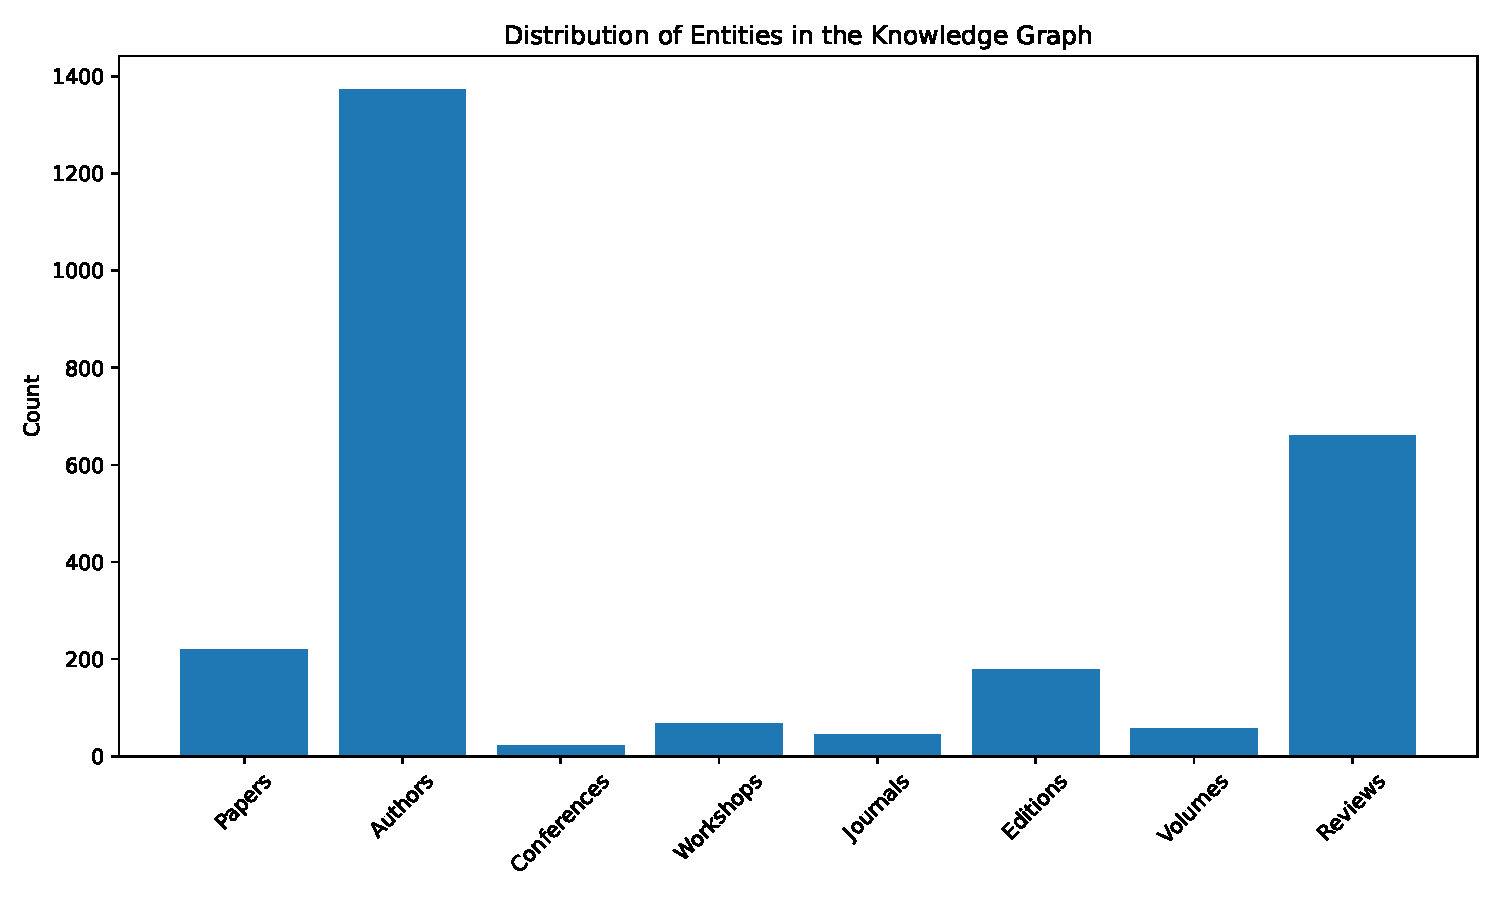
\includegraphics[width=\textwidth]{img/entity_distribution.pdf}
    \caption{Distribution of entities in the knowledge graph. The plot shows the count of each entity type, providing insight into the scale and composition of the knowledge graph.}
    \label{fig:entity_dist}
\end{figure}

The relationships between entities are shown in Figure \ref{fig:relationship_dist}, which illustrates the frequency of different types of connections in the knowledge graph. This helps us understand the density and nature of the relationships in our graph.

\begin{figure}[H]
    \centering
    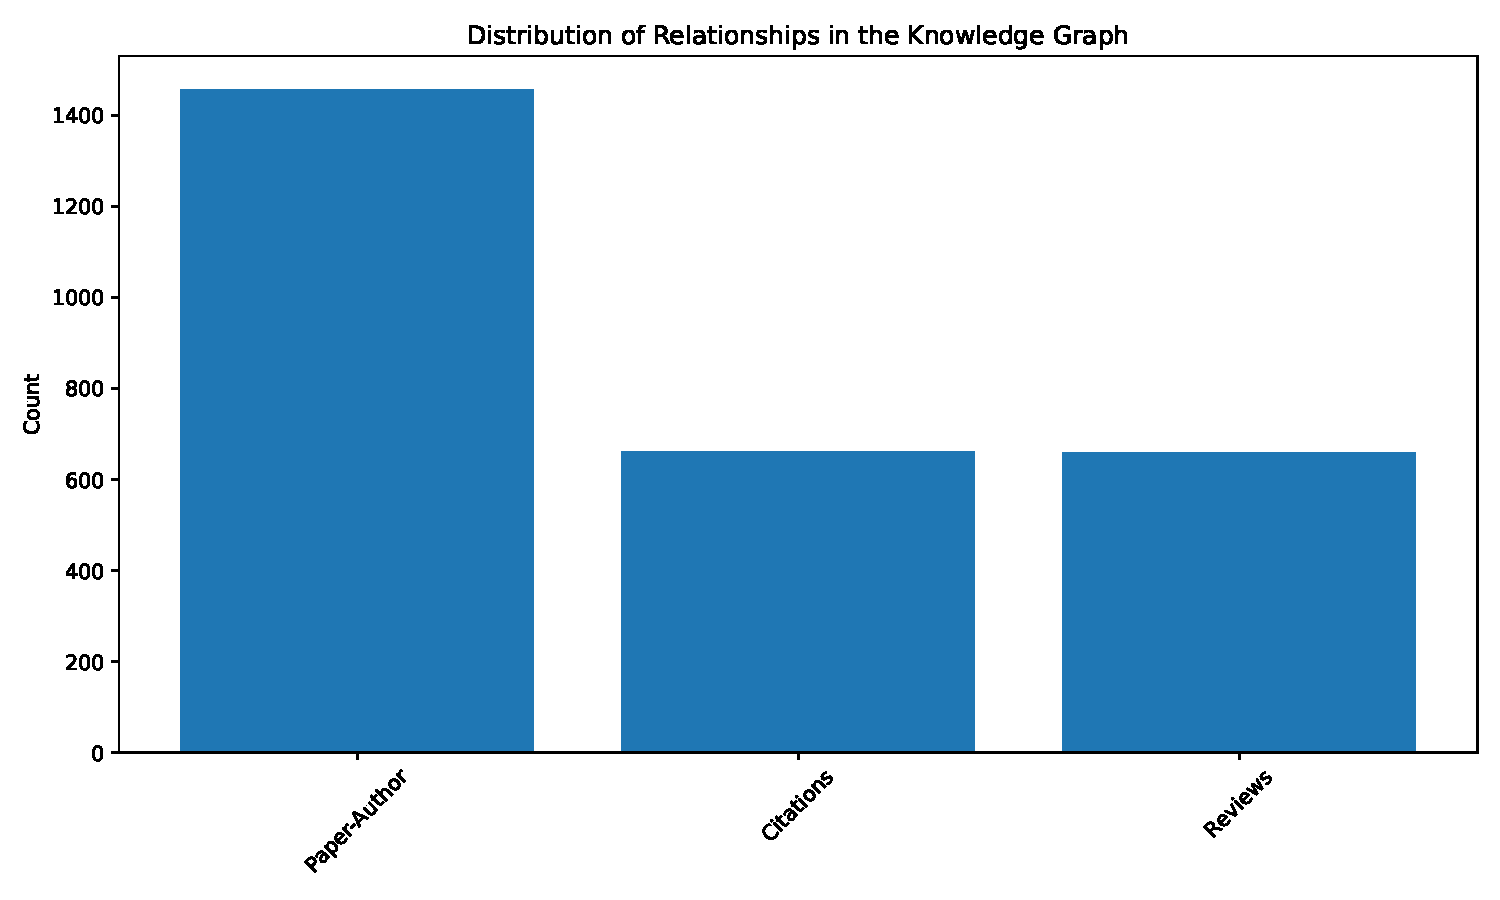
\includegraphics[width=\textwidth]{img/relationship_distribution.pdf}
    \caption{Distribution of relationships in the knowledge graph. The plot shows the count of different types of relationships, highlighting the most common connections between entities.}
    \label{fig:relationship_dist}
\end{figure}

The distribution of publication venues is shown in Figure \ref{fig:venue_dist}, which provides insight into the balance between different types of publication outlets in our dataset.

\begin{figure}[H]
    \centering
    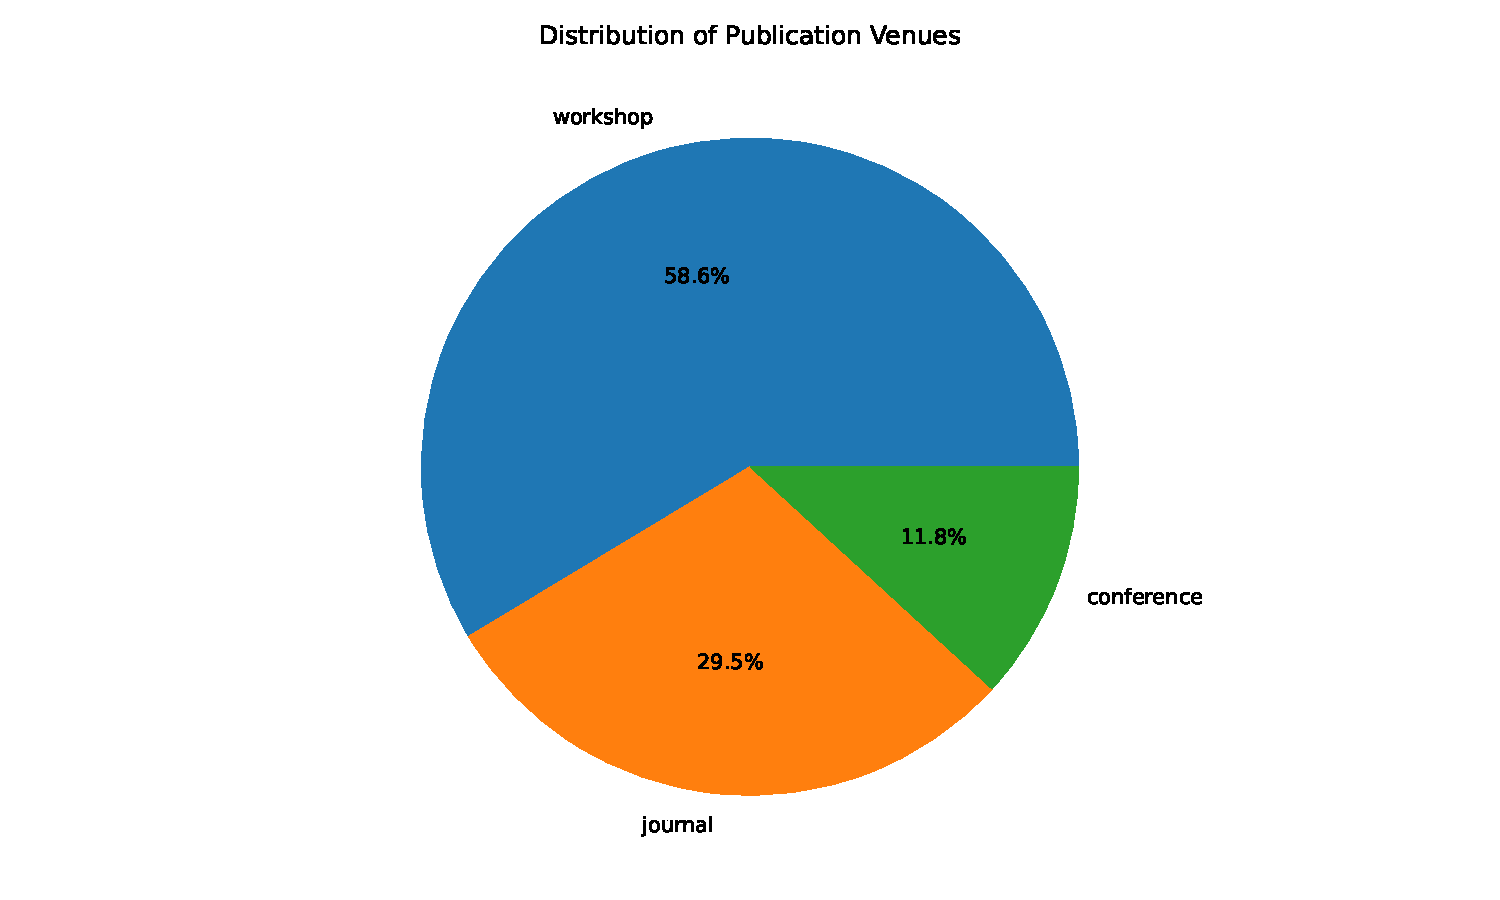
\includegraphics[width=\textwidth]{img/venue_distribution.pdf}
    \caption{Distribution of publication venues. The pie chart shows the proportion of papers published in different types of venues (conferences, workshops, and journals).}
    \label{fig:venue_dist}
\end{figure}

The temporal distribution of papers is shown in Figure \ref{fig:year_dist}, which helps us understand the time span covered by our knowledge graph and any trends in publication frequency.

\begin{figure}[H]
    \centering
    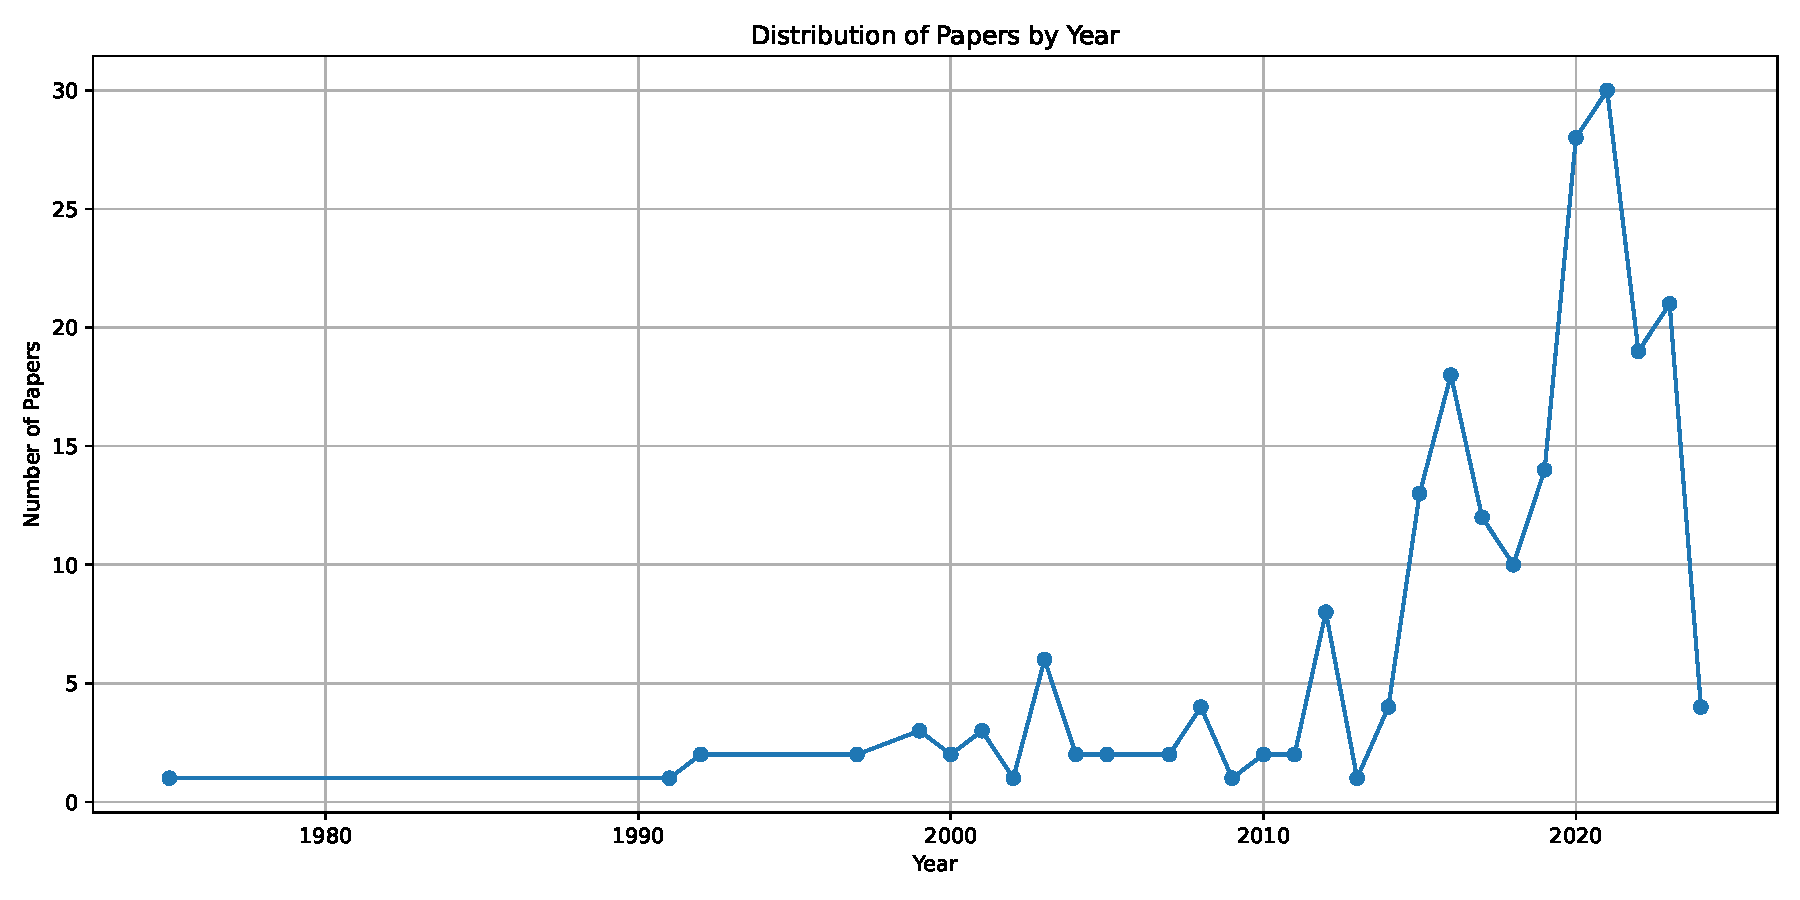
\includegraphics[width=\textwidth]{img/year_distribution.pdf}
    \caption{Distribution of papers by year. The line plot shows the number of papers published each year, revealing trends in publication frequency over time.}
    \label{fig:year_dist}
\end{figure}

Finally, Figure \ref{fig:keyword_dist} shows the most common keywords in the papers, providing insight into the main research topics covered in our knowledge graph.

\begin{figure}[H]
    \centering
    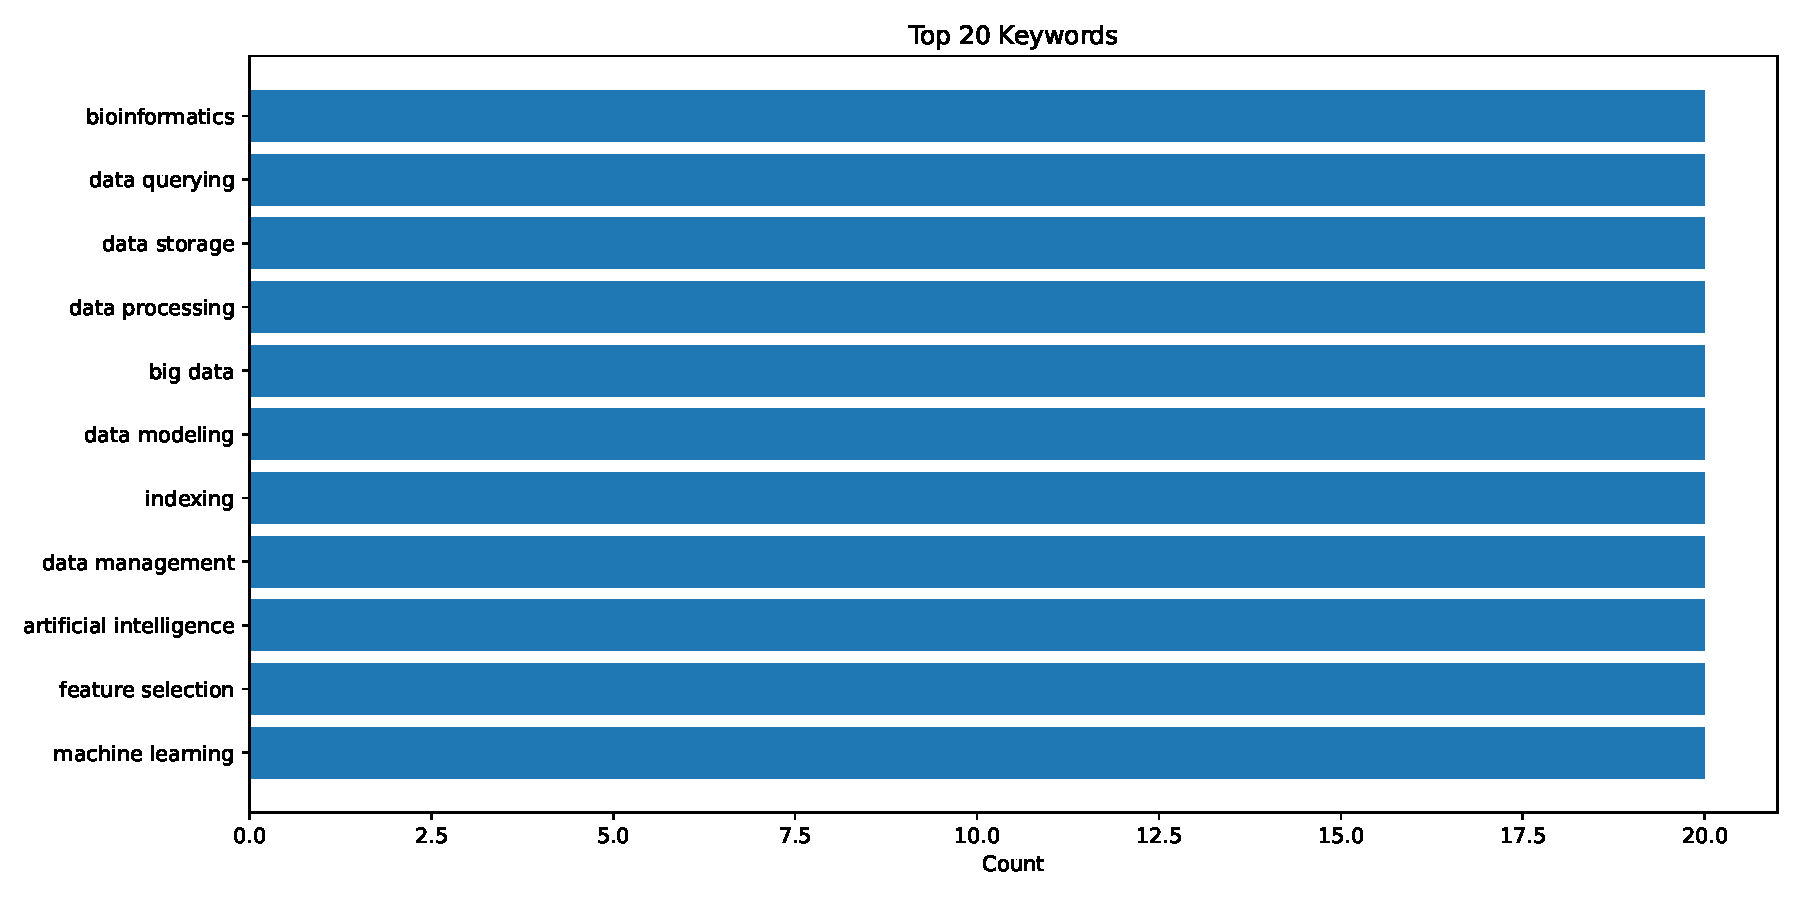
\includegraphics[width=\textwidth]{img/keyword_distribution.pdf}
    \caption{Top 20 keywords in the papers. The horizontal bar chart shows the most frequently occurring keywords, indicating the main research topics in the knowledge graph.}
    \label{fig:keyword_dist}
\end{figure}

These statistics provide valuable insights into the structure and content of our knowledge graph, helping us understand its scale, composition, and the relationships between different entities.

\subsection{Assumptions and Design Decisions}

The implementation makes several key assumptions and design decisions to handle the complexity of the academic publication domain. First, we assume that each paper can be published in exactly one venue (either a conference/workshop edition or a journal volume). This assumption simplifies the relationship structure while maintaining the semantic accuracy of the knowledge graph.

For topics, we assume that keywords are case-sensitive and that whitespace should be preserved. This decision allows for more precise topic matching and querying. The implementation also assumes that keywords are comma-separated in the input data, with each keyword potentially containing internal spaces.

The implementation assumes that author IDs are unique across the entire dataset, allowing for consistent author identification even when the same author appears in multiple papers. This assumption is crucial for maintaining the integrity of author-related relationships.

For temporal data, we assume that years are represented as integers and are valid calendar years. This assumption allows for proper typing of temporal data in the knowledge graph and enables temporal reasoning.

The implementation assumes that each review is uniquely identified by the combination of paper ID and reviewer ID. This assumption allows for proper handling of multiple reviews for the same paper by different reviewers.

Finally, the implementation assumes that the CSV files are properly formatted and that the data types of each column are consistent with their expected usage in the knowledge graph. This includes proper handling of numeric IDs, string values for names and titles, and boolean values for flags like corresponding author status.

These assumptions and design decisions, combined with the robust data validation, ensure that the resulting knowledge graph is both semantically accurate and practically useful for querying and analysis.

\subsection{Querying the Ontology}

To demonstrate the benefits of having an explicit TBOX and enabling reasoning in our knowledge graph, we created two SPARQL queries that showcase different aspects of our ontology.

\subsubsection{Query 1: Finding Corresponding Authors}

The first query demonstrates how reasoning helps us find all papers and their corresponding authors, taking advantage of the subproperty relationship between \texttt{hasCorrespondingAuthor} and \texttt{hasAuthor}:

\begin{lstlisting}[language=SQL]
PREFIX pub: <http://example.org/publication/>
PREFIX rdf: <http://www.w3.org/1999/02/22-rdf-syntax-ns#>
PREFIX rdfs: <http://www.w3.org/2000/01/rdf-schema#>

SELECT DISTINCT ?paper ?paperTitle ?author ?authorName
WHERE {
    ?paper rdf:type pub:Paper .
    ?paper rdfs:label ?paperTitle .
    ?paper pub:hasCorrespondingAuthor ?author .
    ?author pub:hasName ?authorName .
}
ORDER BY ?paperTitle
\end{lstlisting}

This query showcases the power of reasoning in several ways:
\begin{itemize}
    \item It uses the \texttt{hasCorrespondingAuthor} subproperty of \texttt{hasAuthor}, allowing us to find all corresponding authors through reasoning
    \item The TBOX helps us understand the relationships between papers and authors by explicitly defining these relationships
    \item The query results show how the ontology structure enables us to easily find specific types of authors (corresponding authors) without having to explicitly store this information in the ABOX
\end{itemize}

\subsubsection{Query 2: Finding Papers in Events}

The second query demonstrates how reasoning helps us find all papers published in conferences or workshops, taking advantage of the event hierarchy:

\begin{lstlisting}[language=SQL]
PREFIX pub: <http://example.org/publication/>
PREFIX rdf: <http://www.w3.org/1999/02/22-rdf-syntax-ns#>
PREFIX rdfs: <http://www.w3.org/2000/01/rdf-schema#>

SELECT DISTINCT ?paper ?paperTitle ?event ?eventName ?year
WHERE {
    ?paper rdf:type pub:Paper .
    ?paper rdfs:label ?paperTitle .
    ?paper pub:isPublishedIn ?edition .
    ?edition rdf:type pub:Edition .
    ?edition pub:hasYear ?year .
    ?event pub:hasEdition ?edition .
    ?event rdfs:label ?eventName .
    {
        ?event rdf:type pub:Conference .
    } UNION {
        ?event rdf:type pub:Workshop .
    }
}
ORDER BY ?year ?eventName ?paperTitle
\end{lstlisting}

This query showcases the power of reasoning in several ways:
\begin{itemize}
    \item It uses the event hierarchy (Conference and Workshop as subclasses of Event) to find papers published in any type of event
    \item The TBOX helps us understand the publication structure by explicitly defining the relationships between papers, editions, and events
    \item The query results show how the ontology structure enables us to easily find papers published in specific types of venues without having to explicitly store this information in the ABOX
\end{itemize}

These queries demonstrate how the explicit TBOX definition and reasoning capabilities of our knowledge graph enable us to:
\begin{itemize}
    \item Find information that is not explicitly stored but can be inferred through the ontology structure
    \item Understand and query the relationships between different entities in a semantic way
    \item Take advantage of the hierarchical structure of our ontology to find related information
\end{itemize}

\section{Knowledge Graph Embeddings}
\subsection{Importing the Data}
[To be filled with data selection and import details]

\subsection{Getting Familiar with KGEs}
[To be filled with KGE model exploration and analysis]

\subsection{Training KGEs}
[To be filled with KGE training experiments and results]

\subsection{Exploiting KGEs}
[To be filled with KGE application details and results]

\end{document} 